kk
\chapter{Arquitetura}

% \begin{figure}[!h]
%  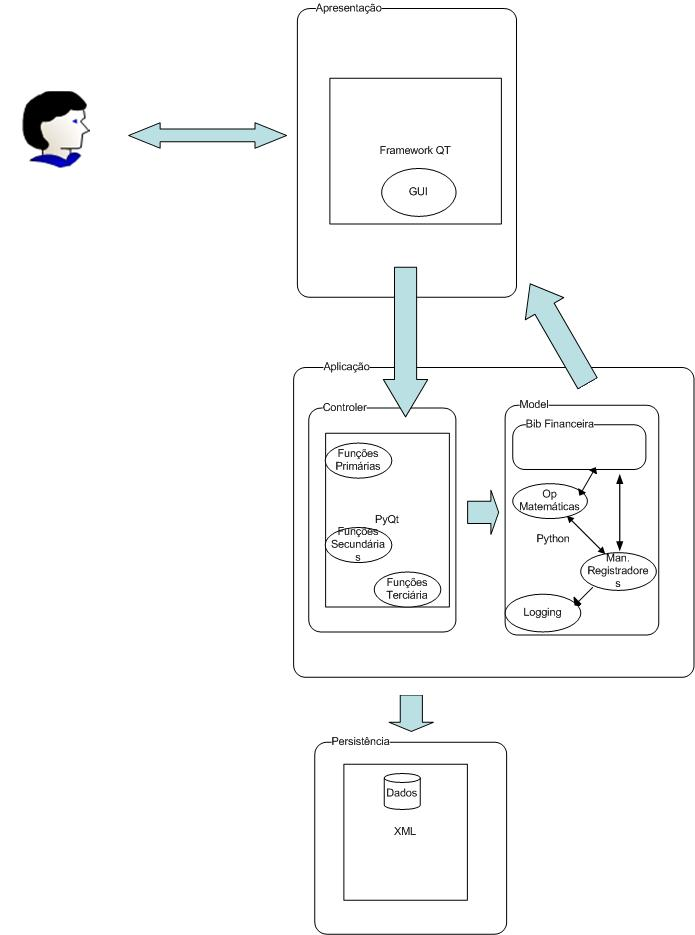
\includegraphics[scale=0.5]{arquitetura.jpg}
%  \caption{\it Projeto arquitetural da aplicação.} \label{fig:arquit}
% \end{figure}
\begin{figure}[!h]
 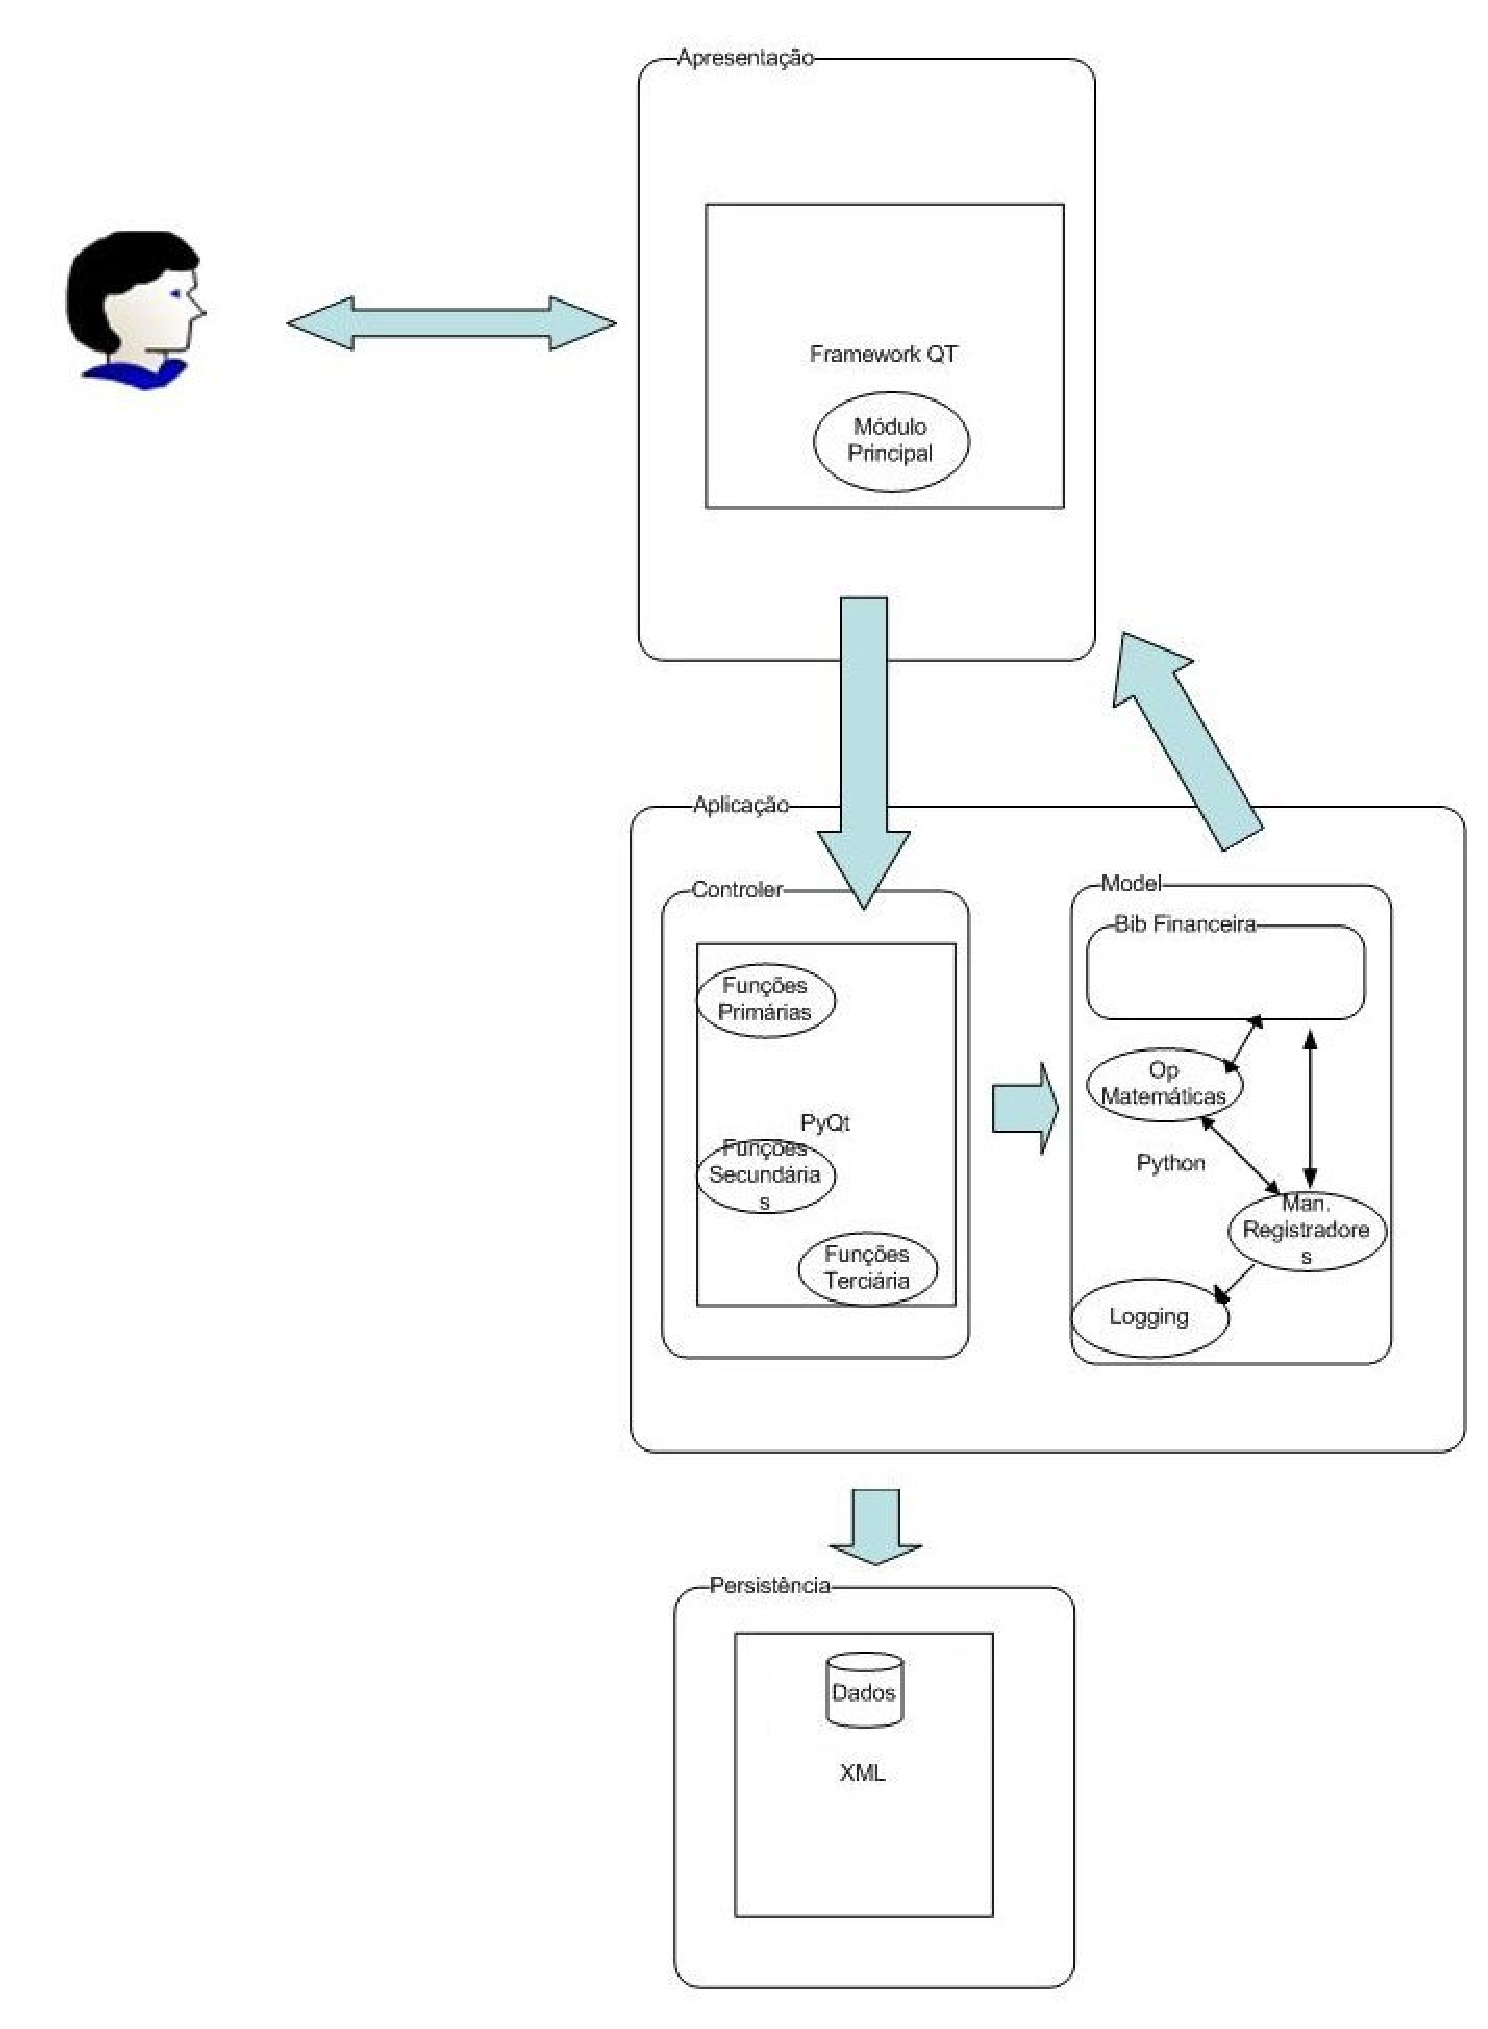
\includegraphics[scale=0.5]{arquitetura.eps}
 \caption{\it Projeto arquitetural da aplicação.} \label{fig:arquit}
\end{figure}

\section{Descrição da Arquitetura}
O sistema proposto foi idealizado para funcionar localmente no dispositivo N800 da Nokia, funcionando no modo monousuário. O sistema pode ser dividido, em três camadas lógicas, que serão conectadas através do padrão MVC \cite{mvc}, conforme pode ser visto na figura \ref{fig:arquit}:
\begin{itemize}
 \item \textbf{Apresentação}: camada que será responsável por lidar com todo aspecto de interface para interação com o usuário.
 \item \textbf{Aplicação}: camada que será responsável por conter toda a lógica do negócio de nossa aplicação, mantendo, assim total desacoplamento com as demais camadas.
 \item \textbf{Persistência}: camada que será responsável por lidar com toda a persistência de dados de mode que eles possam ser usados posteriormente íntegros.
\end{itemize}
Vale lembrar que toda a comunicação entre essas camadas, bem como entre os diversos módulos internos as mesmas, é realizada através de um conjunto de interfaces bem definidas, buscando assim, garantir flexibilidade e baixo acoplamento, bem como um eventual reuso e/ou substituição da biblioteca financeira em questão. A separação estre os módulos se deu da forma mais simplificada possível para que não existisse maior sobrecarga que pudesse influenciar drasticamente o tempo de resposta desejados para as iterações com o usuário da aplicação, este foi um dos requisitos não-funcionais especificados na fase de análise.
Outro ponto importante a se destacar é o uso do paradigma OO, bem como do uso de scripts, dada à escolha da linguagem Python para o desenvolvimento da Camada de Aplicação.

\subsection{Camada de Apresentação}
O sistema será acessado localmente por um único usuário via uma interface similar a da calculadora financeira que estamos usando como base, tendo a adição de menus de auxílio para uso do sistema e uma opção de finalização da aplicação. É importante destacar ainda que toda entrada realizada pelo usuário se dará através da interface touch-screen disponibilizada pelo dispositivo selecionado.
Para o desenvolvimento dessa camada faremos uso do Framework QT, com auxílio da ferramenta de design gráfico QT Designer. É de suma importância aqui o desenvolvimento de packages no que diz respeito aos componentes visuais da calculadora, por exemplo, os botões da mesma.

\subsection{Camada de Aplicação}
Como dito anteriormente, essa camada é responsável por toda a lógica de negócio de nosso sistema e foi desenvolvida em Python devido a suas vantagens na manipulação de números.
Dentre os principais componentes desta camada podemos dar destaque à biblioteca financeira (também desenvolvida por esta equipe com o foco de ser um módulo importável que contenha essencialmente funcionalidades financeiras), ao módulo de operações matemáticas, ao módulo de gerenciamento dos registradores existentes (responsável por fornecer os dados a serem persistidos) e ao módulo de comunicação com a interface da calculadora.
 Dentro dessa camada podemos destacar que as interações ocorrem em duas etapas:
\begin{enumerate}
 \item Numa primeira etapa teremos a comunicação dessa camada com a camada de apresentação do sistema através dos controladores, fazendo estes uso dos bindings em PyQt e sendo subdivididos de acordo com as funcionalidade providas por cada tecla.
 \item Numa segunda etapa teremos:	
 \begin{itemize}
  \item \begin{itemize}
         \item A comunicação dos módulos controladores com o restante da lógica da aplicação, fazendo uso das funcionalidades da biblioteca financeira, do módulo matemático e manipulando os seus registradores.
	 \item A interação entre os registradores e a biblioteca, onde os primeiros podem fornecer entradas para a última, a interação entre os registradores e o módulo matemático e a interação entre o módulo matemático e a biblioteca.
        \end{itemize}
 \end{itemize}
\end{enumerate}

\subsection{Camada de Persistência}
A persistência dos dados relativos aos registradores é realizada através do uso de arquivos. Os dados que forem armazenados nos arquivos deverão ser recarregados sempre que houver a inicialização da aplicação, demandando, assim, pouca interação com o disco nesse sentido.
Outro aspecto relevante a ser considerada aqui é a segurança do sistema.  Devido à natureza do sistema focamos nos aspectos de integridade dos dados manipulados, fazendo com que os arquivos utilizados fossem armazenados de forma oculta ao usuário, evitando, assim, alterações dos mesmos por parte deste.

\subsection{\textit{Packing}}
Foi tomada a decisão de distribuir a aplicação através de um arquivo de instalação de extensão .deb, simplificanco assim a maneira de intalação do software. Tal arquivo poderá ser obtido por download de certo servidor web que será escolhido pela equipe em conjundo com o cliente.

\subsection{Pontos Adicionais}
Com relação à integração com outras aplicações, é do interesse da equipe que a biblioteca financeira desenvolvida possa vir a ser usada por outros desenvolvedores como um dos vários módulos que auxiliem sua aplicação específica.
Por fim, todo nosso desenvolvimento foi guiado pelo padrão de operações que é usado pela HP12-C que é a Notação Polonesa Reversa, ou Inversa segundo alguns autores \cite{NPR}





